\section{Model and evidence}
\begin{frame}{A production function}
Output depends on capital and labour:
\begin{equation}\econOutput = A K^{\alpha} L^{1-\alpha}\label{eq:production}\end{equation}
\pause
\begin{itemize}
\item For this example, $A=1$ and $\alpha=0.3$.
\item Equation \eqref{eq:production} is an illustration, not an estimated relationship.
\end{itemize}
\begin{center}
\begin{tabular}{lrr}\toprule
Scenario & Capital $K$ & Labour $L$ \\\midrule
Baseline & 100 & 50 \\
Alternative & 120 & 50 \\\bottomrule
\end{tabular}
\end{center}
\end{frame}
\begin{frame}{Illustrative output}
\begin{center}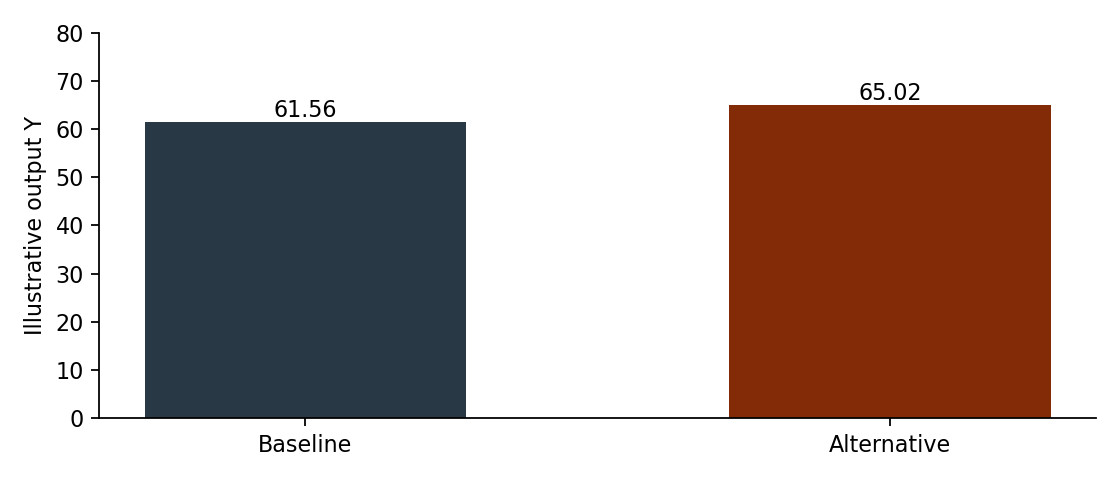
\includegraphics[width=.68\linewidth]{figures/output.png}\end{center}
\footnotesize Source: invented teaching values; no empirical claim. See \citet{example}.
\end{frame}
\section{Human review}
\begin{frame}{Check the conversion}
\begin{center}
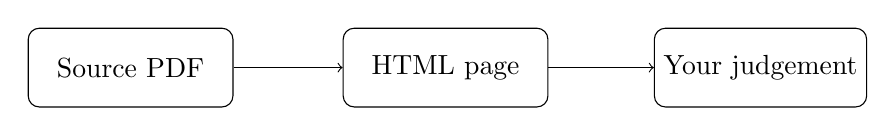
\begin{tikzpicture}[every node/.style={draw,rounded corners,minimum width=2.6cm,minimum height=1cm}]
\node (source) at (0,0) {Source PDF};
\node (html) at (4,0) {HTML page};
\node (check) at (8,0) {Your judgement};
\draw[->] (source) -- (html);\draw[->] (html) -- (check);
\end{tikzpicture}
\end{center}
\begin{itemize}
\item Compare maths, figures, tables and slide order.
\item Change one conversion rule; rerun and check again.
\end{itemize}
\note{The diagram can be rendered from the PDF if it cannot be converted directly.}
\end{frame}
\begin{frame}{References}
\bibliographystyle{plainnat}\bibliography{references}
\end{frame}
